\section{インタビュー調査}
% \section{Formative Study}
\label{section:Formative_Study}

\subsection{プログラマの要望調査}

実際のソフトウェア開発でのコード理解における障壁を調査するために,我々はIT企業に所属する5人のプログラマ(PA1--5,全員男性)にインタビューを行った.
実験参加者は全員,ソフトウェア開発プロジェクトにおいてGitHubを日常的に利用していた.
インタビューでは実験参加者がコード理解をどのように行い,その際にどのような障壁が存在するのかを重点的に尋ねた.


% システムのデザインの方向性を決定するために,我々は5人の\shibato{プロのプログラマー}{professional programmer}(PA1--5, all 全員男性)に\shibato{事前インタビュー調査}{formative study}を行なった.
% 実験参加者は全員,仕事において日常的にGitHubを利用している.
% コード理解の重要性は既に広く知られているため,このインタビューは実験参加者がコード理解をどのように行い,その際にどのような障壁が存在するのかを明らかにすることとした.

% To be informed of the interface design, we conducted a formative interview study with five professional programmers (PA1--5, all male).
% All participants regularly used GitHub in their work environments.
% Because it is already well known how important code comprehension is in general, our interview focused on how they normally developed code understanding and what issues they encountered.
% As a result, this formative study revealed the following two findings.

%Our interview study took approximately one hour.
%The participants were offered a compensation of approximately 15 USD in the local currency at the end of the interview.
%As we conducted our interviews in a local language, we translated quotes in English for the following report.


% \begin{figure*}[t]
% \centering
%   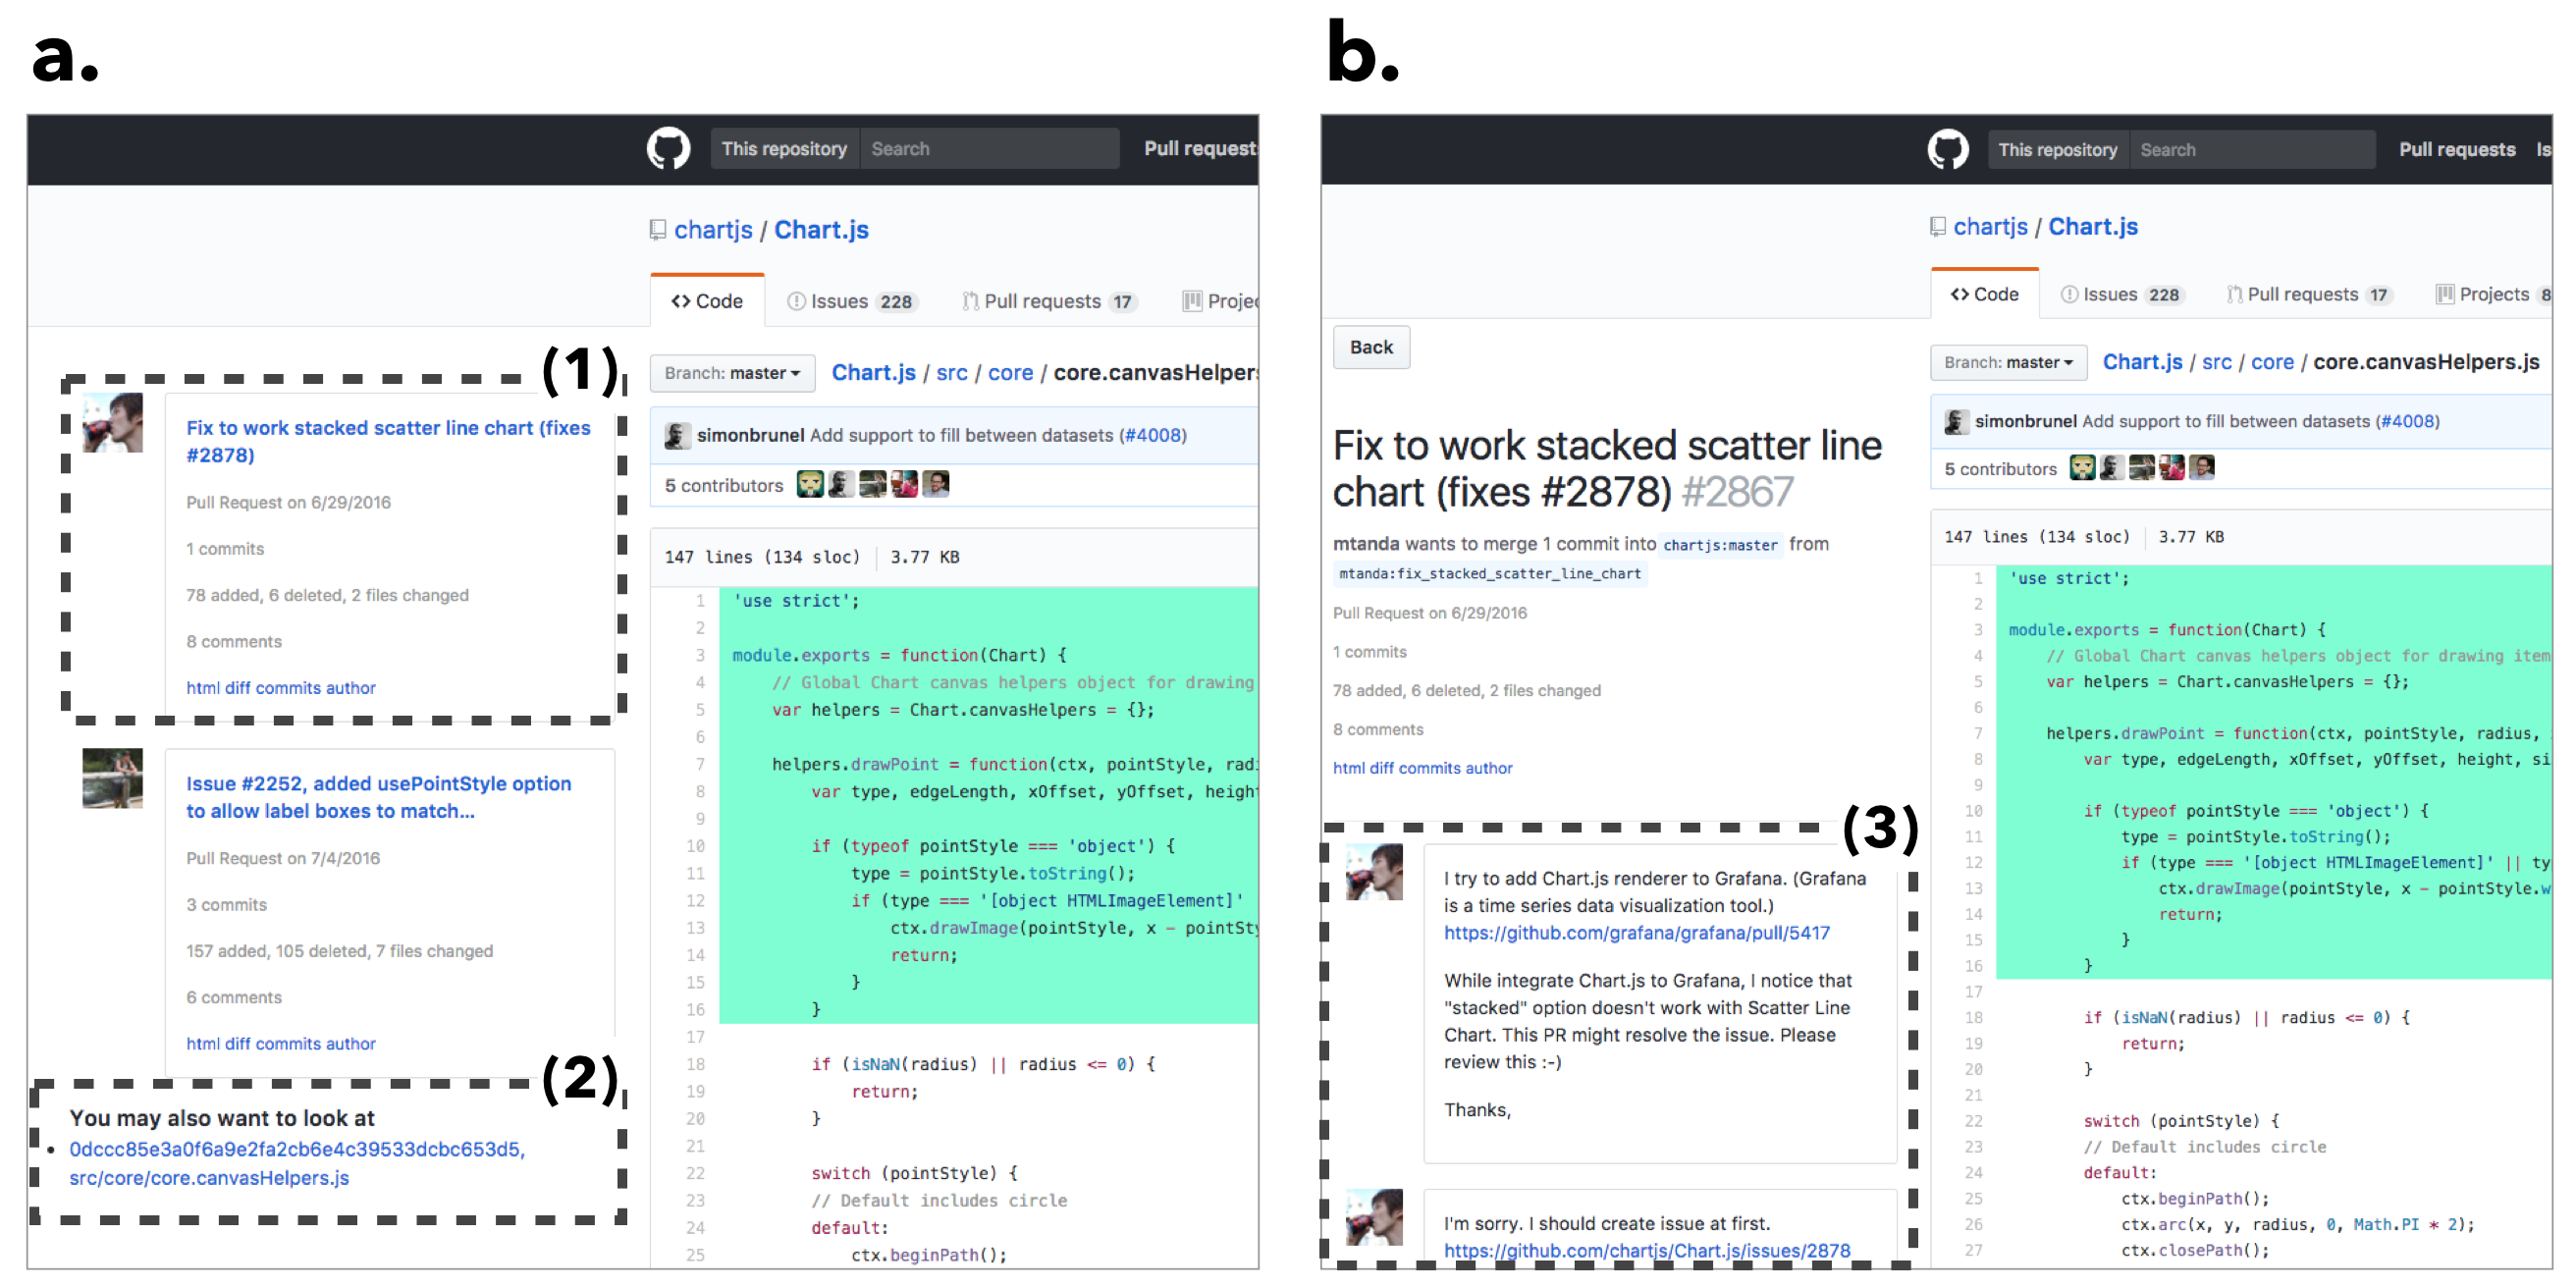
\includegraphics[width=2.0\columnwidth]{interface/CodeGlass.png}
%   \caption{The CodeGlass interface displays a series of pull requests associated with the user-selected code piece (highlighted in light green) in the chronological order. (1) Each pull request is summarized in a separate box. A summary shows the title of a pull request, its ID, and the numbers of commits, lines and files changed, and comments as well as links for additional information. (2) CodeGlass also suggests commits that are not included above but can be relevant if there exists any. When clicking one of them, the user can view the version associated with the selected commit and further investigate how code has been developed. (3) When the user clicks the title, CodeGlass presents review comments in the selected pull request.}~\label{fig:WebInterface}
% \end{figure*}


\subsubsection*{開発背景を理解する難しさ}
% \subsection{Burden for Collecting Development Contexts}

% チーム開発においては,実装やコードレビューのために他の開発者が実装したソースコードを理解する必要がある.
% しかし,他人が書いたコードの理解には大変な労力を要する.
% PA1はコードレビュー時にコード変更を理解することが困難となっていると指摘した.

% In collaborative development, understanding code written by others is crucial.
% However, effort for code comprehension can be substantial. 
% PA1 stated how tedious it can be when he was involved in code review.

% \myquote{(コードレビューにおいて,人のコードを読む事は)まじめにやるとコード書くのと同じくらい時間かかるんですよ}{PA1}
% \myquote{(In code review,) Understanding others' code can be as time-consuming as writing code if you do it seriously.}{PA1}

チーム開発においては,実装やコードレビューのために他の開発者が実装したコードを理解する必要があるが,他人が書いたコードの理解には大変な労力を要する.
また,実際のソフトウェア開発におけるコード理解では,コードの実装内容だけでなく,なぜ実装されたのかという開発背景も把握することが重要である.
%何故なら,実際のソフトウェア開発では厳格な締め切りやビジネス上の理由により,常に最善の実装方法が選択されるとは限らないからである\shibato{}{cite}.
PA1は,コードレビューにおいて背景知識の不足がコード理解における問題の一つである事を以下のように指摘した.
%特にチームの新しい開発メンバーにとってはこの問題は深刻である.

% Code comprehension includes understanding the context of how the code has been developed in addition to what it executes.
% PA1 mentioned a particular issue related to code review caused by the lack of context understanding.
% Such development contexts is important particular for new team members.

\myquote{プロダクトの背景がわからないことが課題となっていて,長く見ている人が初めてそのチーム内でレビューできるようになっていて,まだやっぱり新入りの人がコードレビューできるような状況までドキュメントが整備されていないし,やっぱり背景理解が難しい.}{PA1}

% \myquote{One issue is the lack of background knowledge about the product. It makes only old members able to perform code review. Documentation is not ready for new members, and they cannot perform code review. It is still difficult for them to understanding the background.}{PA1}

% This problem becomes more prominent when new team members were on board.
% P1 mentioned that he frequently observed that new team members struggled on collecting background information.

% % \myquote{やっぱりコードの背景というか,コンテキストがわからないので,そこはなんかわかんないのは当たり前だと思う}{P1}
% \myquote{It is unsurprising that new team members do not understand the project well because they do not know its context or background.}{P1}

% \myquote{どういう背景があってこのコードを実装したのかが書いてあると嬉しい.}{P3}
%\myquote{It would be great if it is clear why this code has been implemented.}{PA3}

% Software documentation is one of the best practices to share knowledge of source code among team developers.
% However, PA5 stated that creating documentation would cause additional overhead in a project, and his team decided not to engage in it.

% % \myquote{チーム内でもドキュメントを作ろうという流れになる事はあります,ありますけど,正直なところあのーそこにさけるパワーは今,ちょっと・・,開発スピードを重視したいので}{P5}
% \myquote{We do have plans to create documentation, but to be honest, we don't have bandwidth for it now. We want to focus on speeding up our development.}{PA5}


\subsubsection*{コード理解のための情報源としてのプルリクエスト}
% \subsection{Pull Requests as an Information Resource}

% Code review was a common activity we observed in our interviews.
% It is one development process where a developer validates code revisions developed by another programmer.
% Bacchelli and Bird~\cite{MotivationOfCodeReview-Bacchelli} reported that while the main motivation for code review was to identify defects, reviewers also expected additional benefits, such as learning alternative solutions or performing knowledge transfer.
% For these multi-faceted benefits, code review becomes an integral part of a modern development process.

% GitHub supports code review through pull requests.
% A pull request includes a description of revisions as well as the actual code changes.
% A reviewer performs merge (or pull in GitHub) when she finds the revisions to be bug-free and legitimate.
% Our participants mentioned that additional effort by developers can greatly facilitate a code review process.
% For instance, a well-written description of a pull request can offer a sufficient amount of information about and reasons for the code changes, supporting reviewers' activities.

%適切にコードレビューを行うためには,開発者がレビュアーにコード変更の内容や開発背景を伝える必要がある.
実験参加者らはコード変更をレビュアーに説明するために,GitHubの機能の一つあるプルリクエストを活用していた.
プルリクエストでは,説明文に目的や内容を記述することで,コード変更をより分かりやすく他の開発者に伝える事が可能となっている.
PA3とPA5は,コードが実装された理由を後から確認するために,開発背景といった情報を含むプルリクエストを参照する事があると指摘した.

% 実験参加者らは,彼らのソフトウェア開発においてGitHubの機能の一つあるプルリクエストを活用していた.
% プルリクエストではコード変更の目的や内容を説明に記述する事が出来る.
% 彼らはプルリクエストの説明文やコメント内にコード理解のための有用な情報が多く存在する事を指摘した.
% 例えばPA3とPA5は,そのコードが実装された理由を理解するためによくプルリクエストを参照していると述べた.


% Our participants regularly used pull requests in their projects as part of a code review process.
% They agreed that comments and logs in pull requests can be useful to obtain information about code. 
% For instance, PA3 and PA5 often referred to past pull requests to understand implementation reasons.

\myquote{それは,実装を見ててこれってどういう意図でこうなってんのとかが,気になった時は,結構プルリクエスト上で議論がなされていることが多いので,それを探しに行くことはあります.}{PA3}
% \myquote{When I have a question about why this implementation was made, I look for pull requests because they often include related discussions.}{PA3}

\myquote{僕はわりと探っちゃうタイプなので,昔どういうことあったんだろうみたいなのは追っちゃう感じですね.}{PA5}
% \myquote{I like digging into code, so I often look for pull requests to see what happened in the past.}{PA5}

% PA1 and PA3 stated that they and their team explicitly described contexts as well as the content of changes.


% % \myquote{重要だと思ってるのは,まあ一個一個何でどういう目的でやるのかっていうのを書くようにしてるんですよね,formatをwhyとwhatを書くようにしている}{P1}
% \myquote{What's important to me is to describe what each change does for what purposes. We have a format (for pull requests) to make sure to write why and what.}{PA1}
% % \myquote{見てもらう人のことは考えて,どういう変更をどういう意図で行ったのかっていうのは,書くようにしている}{P3}
% \myquote{I always think of the reader, and clearly write what changes I have made for what purposes.}{PA3}

% Similar to general code comprehension, understanding development contexts is important for code review.
% P4 mentioned that the problem arises when he asked external developers to perform code review. 

% %\myquote{他のチームにレビューを頼む時に,プロダクトの背景がわからないことが課題となっていて,長く見ている人が初めてそのチーム内でレビューできるようになっていて,まだやっぱり新入りの人がコードレビューできるような状況までドキュメントが整備されていないし,やっぱり背景理解が難しい.}{P4}

% \myquote{When I have to ask someone in another team to review, the problem is that he does not have background knowledge about the project. People cannot do proper reviews until they are in a team for a long time.}{P4}




% \subsection{Summary}
% Our interview study thus highlights the following findings.

% \begin{itemize}
% \setlength{\parskip}{1mm}
% \setlength{\itemsep}{0mm}
% %\item Developers are frequently required to understand codes before performing further actions (e.g., reviewing and making revisions).
% \item Developers desire to obtain relevant information about the portion of code they are investigating for understanding, but they do not always have appropriate support.
% \item Past pull requests can be useful to understand the context or reasons of code changes.
% \end{itemize}

以上より,プルリクエストの説明文にはコード理解において有用な情報が含まれている可能性があり,実際に開発現場で利用されることがあることを確認した.
この発見により,プルリクエストをコード理解に活用するシステムを構築することを考えるに至った.

% These findings led us to a hypothesis that improving accessibility to relevant pull requests would support comprehension of code portions.

\subsection{既存技術の問題点調査}
% \section{Study on Existing Command-based Tools}
% %Our interview with professional programmers revealed that past pull requests can be a useful resource for understanding code.

続いて我々は,既存のツール,特にtig\footnote{\url{https://github.com/jonas/tig}}とrecursive-blame\footnote{\url{https://github.com/scottgonzalez/recursive-blame}}がコード理解の支援においてどのように不十分であるかを調査した.
% 続いて我々は,何故プルリクエストを活用したコード理解を既存のツールでは実現できていないのかを調査することとした.
% 続いて我々は,コード断片の理解を支援でき得る既存のツールの評価を行った.
tigはgit blameのコマンドを再帰的に実行できるコマンドラインインターフェースであり,recursive-blameは特定のキーワードを含む過去のコード変更を抽出することができるコマンドである.
%tigとrecursive-blameの技術的先行調査を行った結果,CodeGlassと異なり,コード断片の追跡を自動で再帰的に行うことができないことが明らかとなった.
%したがって,CodeGlassとtigおよびrecursive-blameを同一の条件下で比較評価を行うことは難しいため,我々は定性的な調査を行うこととした.
本調査ではGitHubのプルリクエストを用いた開発経験のある7人の学生(PB1--7)にインタビューを行った.
インタビューではまずtigまたはrecursive-blameを用いてコード断片の調査を行ってもらい,その後2つのツールに対する使用感を尋ねた.
その結果,既存のツールでは過去のプルリクエストをコード理解のために活用することができない2つの理由が明らかとなった.

% We further examined why existing tools cannot support extraction of past pull requests well.
% Specifically, we looked into tig\footnote{\url{https://github.com/jonas/tig}} and recursive-blame\footnote{\url{https://github.com/scottgonzalez/recursive-blame}}.
% Although we initially considered a comparative study, we found a large discrepancy in backtracking capability between CodeGlass and these tools as the following results suggest.
% We thus concluded that a comparison under fair conditions would be difficult, and decided to conduct a qualitative study instead.



% To understand how these tools would be useful even for novice developers, we recruited seven university students (PC1--7) who had sufficient experience in GitHub and pull-request-based development.
% We asked the participants to find pull requests related to portions of code in Chart.js given by the experimenter using tig and recursive-blame.
% We then conducted a short interview to understand the user experience of these tools.
% As a result, we found two major issues that existing tools cannot address well.

% \subsubsection{Limited commit backtracking capability}
\subsubsection*{コード断片追跡機能の限界}

%PC1 stated that recursive-blame often cannot trace back the history when the specified pattern of code was changed.

%\myquoute{単純に名前が変わったりすると追えないとかがあるから,基本的にある程度あいまい検索ができるといいんだと思う}{PC}

%Tig finds the latest commit and version containing a change on the user-selected line of code using the git-blame command.
%However, it may fail to determine the commit when changes are substantial as P6 stated:

% % \myquote{色々書きかえると結構すぐ追えなくなりますよね}{P6}

% %The tools tested only take constrained input for search (a line of code and a regular expression or keyword in tig and recursive-blame, respectively).
% %This limitation prevented our participants from correctly identifying relevant pull requests.


実験参加者らは,既存のツールではコード断片が削除または移動された際に,開発履歴の情報が抽出できなくなることを指摘した.
これはコード断片が削除または移動された場合,既存のツールでは単にコード断片が存在しないことのみが表示されるからである.
% Our participants pointed out that existing tools cannot clearly inform whether the portion of interest was completely deleted or moved from a different part (e.g., by refactoring).
% This is because the tools only indicate the deletion of such a portion, and additional manual confirmation is necessary.

\myquote{違う名前や使い方が変わったときに,じゃあ何になったんだろうというってのを探すためには,前の名前しか知らないときは自分で探さないといけない.削除なのか,変更なのかわからないのが今のツールではわからない.}{PB4}
% \myquote{For example, when I found revisions on names or usage, I have to eyeball to figure out whether deletion or changes had occurred, which  these tools cannot tell me.}{PC4}


% \subsubsection{Limited interaction}
\subsubsection*{インタラクションの限界}

tigとrecursive-blameでは,追跡するコードの行やキーワードを繰り返し指定することで,関連する過去のプルリクエストを特定することができる.
しかし,プルリクエストを特定した際に提示される情報には,説明文やコメントが含まれていないため,コードの理解につながると限らないことが指摘された.

% Although the two tools can identify past pull requests, their interfaces do not offer an overview of descriptions and comments.
% This diminishes the utility of the tools as code comprehension support.
%Our participants commented that an overview of relevant pull requests would be desirable.

\myquote{全部やった後にさ,descriptionなかったらさ,なんやねんって感じやん.多分descriptionが一番大事だから,はずれだったらすぐ次のを見せてほしい.}{PB2}
% \myquote{I think descriptions are the most important. So I want to have a way to quickly move on to the next if the current pull request isn't useful.}{PC2}

%\myquote{一度にいくつか(プルリクエストを)見られればうれしいかなと思う,まとめて勝手に深追いしてほしい}{PC4}
% \myquote{If I can see multiple pull requests at one time, that would be great. A system should just automatically backtrack for me.}{PC4}

% %P5 wanted a system that simultaneously provides code and description in pull requests.
% % \myquoute{コードと説明文の二つを同時に表示してあげるインタフェースがあると,使いやすいインターフェースかなと思うしとっつきやすいかなと思う}{P5}

tigではコード中の1行を,recursive-blameではキーワードもしくはコード1行のみを検索に利用できるが,コード理解においては複数行の選択が必要であることを指摘していた.

% Tig and recursive-blame take a single line of code and a keyword in the regular expression form for search, respectively.
% Our participants complained that this search method does not fit to their expected use cases, and the tools should support selection of multiple lines or code pieces.

\myquote{コード読んでて,この行だけわかんないってなることはないから.}{PB1}
% \myquote{It's unlikely that I do not understand only this particular line when I read code.}{PC1}

\myquote{このifの中みたいな,意味のある単位で見たい.ifの行自体は別にそれほど興味ないし中身が大事かな,みたいな.}{PB5}
% \myquote{I want to look into a meaningful chunk, such as code inside this if block. I am not really interested in the line of the if statement itself.}{PC5}

% %\subsubsection{Limited search capability}
% % \myquoute{キーワードで検索は面倒というか,自分が思ったところを検索出来ているのか不安.どこが引っかかるか直感的じゃないから,tigのほうがいいかも}{P3}

\subsection{まとめ}

% Our literature survey identified the following five information categories developers seek in code comprehension:
我々が行った関連研究の調査では,コード理解に重要な情報は以下の5つに大別されることがわかった.



\begin{itemize}
\setlength{\itemsep}{0cm}
%\setlength{\leftskip}{-3mm}
\item \textbf{Execution}: そのコードが何を実行するのか~\cite{Information_Needs_in_Collocated_Software_Development_Teams}.
\item \textbf{Rationale}: 何故そのコードが実装されたのか~\cite{Information_Needs_in_Collocated_Software_Development_Teams}.
\item \textbf{History}: そのコードがどのように変更されてきたのか~\cite{Chronicler}.
\item \textbf{Contributor}: 誰がそのコードの実装に関わったのか~\cite{Who_can_help_me_with_this_source_code_change}.
\item \textbf{Usage}: そのコードがどこでどのように使用されるのか~\cite{Six_Learning_Barriers_in_End_User_Programming_Systems}.
\end{itemize}

% \begin{itemize}
% \setlength{\itemsep}{0cm}
% \setlength{\leftskip}{-3mm}
% \item \textbf{Execution}: What the given code piece executes~\cite{Information_Needs_in_Collocated_Software_Development_Teams}.
% \item \textbf{Rationale}: Why the given code piece is implemented in the way it is~\cite{Information_Needs_in_Collocated_Software_Development_Teams}.
% \item \textbf{History}: How the given code piece has been evolved~\cite{Chronicler}.
% \item \textbf{Contributor}: Who was involved in the implementation of the given code piece~\cite{Who_can_help_me_with_this_source_code_change}.
% \item \textbf{Usage}: Where and how the given code piece is used in a project~\cite{Six_Learning_Barriers_in_End_User_Programming_Systems}.
% \end{itemize}

我々のインタビュー調査により,プログラマが特にコード変更に関する詳細な説明と開発背景の知識をプルリクエストに求めていること,さらに既存のツールではそれが十分に支援されないことが明らかとなった.
したがって,我々が構築するシステムにおいては特にExecutionとRationaleに関する情報収集を支援すべきであると考えた.









